\documentclass{article}
\usepackage[paperwidth=16cm,paperheight=9cm,margin=5pt]{geometry}
\usepackage{tikz}
\usepackage[OT1]{fontenc}
\usepackage{lmodern}
\usepackage{amsmath,amssymb}
\usetikzlibrary{arrows}
\newcommand{\PP}{\mathbb{P}}
\renewcommand{\AA}{\mathbb{A}}
\DeclareMathOperator{\Hilb}{Hilb}
\DeclareMathOperator{\Bl}{Bl}
\definecolor{whs black}{HTML}{151B22}
\definecolor{whsRed}{HTML}{B42A32}
\definecolor{whsGreen}{HTML}{17733E}
\definecolor{skyBlue}{HTML}{87CEEB}
\begin{document}
\pagestyle{empty}
\noindent
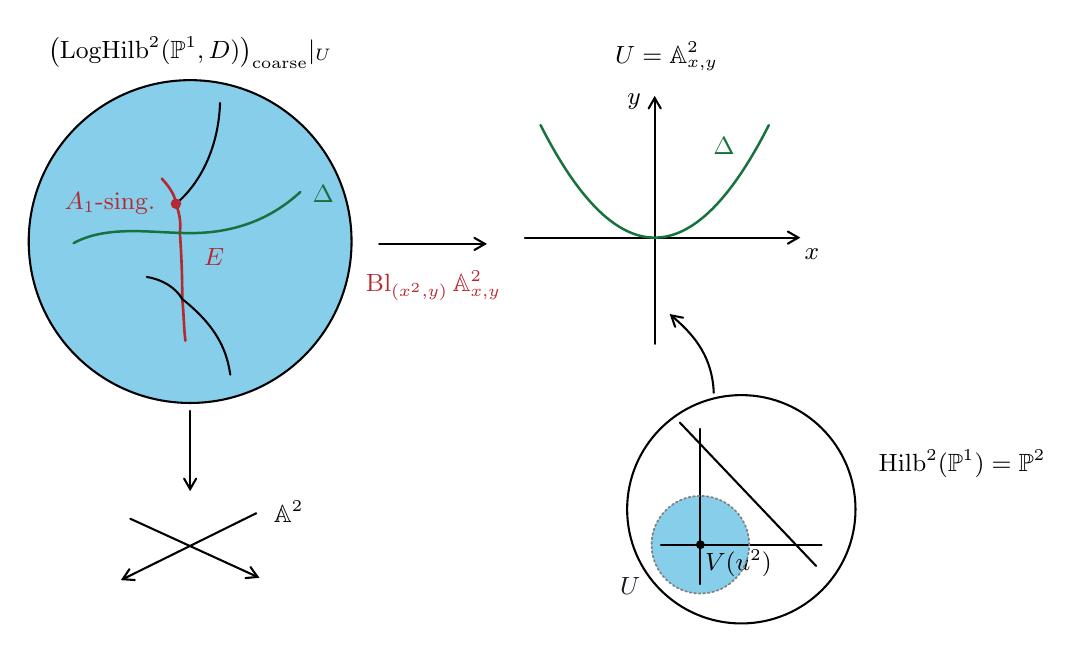
\begin{tikzpicture}[
  x=1cm, y=1cm,
  font=\small,
  line cap=round, line join=round,
  >=angle 60,
  whs red/.style={draw=whsRed, line width=.95pt},
  whs green/.style={draw=whsGreen, line width=.9pt},
  whs black/.style={draw=black, line width=.75pt}
]

% Left: local coarse logarithmic model. Source label D is preserved.
\begin{scope}[shift={(2.65,4.95)}]
  \draw[whs black,fill=skyBlue] (0,0) circle[radius=2.05];
  \node[text=black] at (0,2.40)
    {$\bigl(\operatorname{LogHilb}^2(\PP^1,D)\bigr)_{\mathrm{coarse}}|_U$};

  \coordinate (q) at (-.18,.48);
  \coordinate (g) at (-.13,.11);
  \coordinate (b) at (-.10,-.73);
  \draw[whs red]
    (-.36,.80)
      .. controls (-.24,.67) and (-.19,.57) .. (q)
      .. controls (-.12,.31) and (-.12,.22) .. (g)
      .. controls (-.11,-.18) and (-.10,-.43) .. (b)
      .. controls (-.08,-.92) and (-.08,-1.10) .. (-.06,-1.26);
  \draw[whs black]
    (.38,1.76)
      .. controls (.36,1.18) and (.12,.73) .. (q);
  \draw[whs black]
    (-.55,-.45)
      .. controls (-.35,-.48) and (-.18,-.59) .. (b)
      .. controls (.38,-1.11) and (.47,-1.43) .. (.51,-1.69);
  \draw[whs green]
    (-1.48,-.02)
      .. controls (-1.08,.20) and (-.54,.12) .. (g)
      .. controls (.53,.08) and (1.02,.28) .. (1.40,.63);
  \fill[whsRed] (q) circle[radius=1.9pt];
  \node[text=whsRed, anchor=east, xshift=-4pt] at (q)
    {$A_1\text{-sing.}$};
  \node[text=whsRed, anchor=west] at (.05,-.20) {$E$};
  \node[text=whsGreen, anchor=west] at (1.43,.61) {$\Delta$};
  \draw[whs black, ->] (0,-2.15) -- (0,-3.17);
  \draw[whs black, ->] (-.76,-3.52) -- (.88,-4.27);
  \draw[whs black, ->] (.84,-3.45) -- (-.88,-4.30);
  \node[anchor=west] at (.94,-3.43) {$\AA^2$};
\end{scope}

\draw[whs black, ->] (5.05,4.92) -- (6.42,4.92);
\node[text=whsRed] at (5.74,4.39)
  {$\Bl_{(x^2,y)}\AA^2_{x,y}$};

% Upper right: symmetric local chart U = A^2_{x,y}.
\begin{scope}[shift={(8.55,5.00)}]
  \node at (.15,2.30) {$U=\AA^2_{x,y}$};
  \draw[whs black, ->] (-1.65,0) -- (1.85,0);
  \draw[whs black, ->] (0,-1.35) -- (0,1.80);
  \node[anchor=north west] at (1.78,-.02) {$x$};
  \node[anchor=east] at (-.05,1.73) {$y$};
  \draw[whs green,domain=-1.45:1.45,samples=70,variable=\t]
    plot ({\t},{0.68*\t*\t});
  \node[text=whsGreen] at (.88,1.17) {$\Delta$};
\end{scope}

\draw[whs black, ->]
  (9.30,3.03)
    .. controls (9.28,3.55) and (8.98,3.82) .. (8.74,4.03);

% Lower right: Hilb^2(P^1) = P^2, with the sky-blue U inside it.
\begin{scope}[shift={(9.65,1.55)}]
  \draw[whs black] (0,0) circle[radius=1.45];
  \coordinate (d) at (-.52,-.45);
  % Fill is drawn before incidence lines, so those lines stay visible.
  \fill[skyBlue] (d) circle[radius=.62];
  \draw[whs black] (-.52,1.02) -- (-.52,-.95);
  \draw[whs black] (-1.02,-.45) -- (1.02,-.45);
  \draw[whs black] (-.78,1.10) -- (.95,-.72);
  \fill (d) circle[radius=1.6pt];
  \node[anchor=north west, inner sep=1.5pt] at (d) {$V(u^2)$};
  \draw[draw=whs black!55,densely dotted,line width=.65pt]
    (d) circle[radius=.62];
  \node[text=whs black, anchor=east] at (-1.16,-.98) {$U$};
  \node[anchor=west] at (1.62,.58)
    {$\Hilb^2(\PP^1)=\PP^2$};
\end{scope}
\end{tikzpicture}
\end{document}
